% -*- compile-command: "pdflatex report.tex"; -*-
\documentclass[a4paper,12pt]{article}
\usepackage[utf8]{inputenc}
\usepackage[english]{babel}
\usepackage{graphicx}
\usepackage{listings}
\usepackage{hyperref}
\lstset{
language=C,
basicstyle=\scriptsize
}

\title{Let it snow}
\author{Christian Luckey \\ Matteus Hemström}


\begin{document}

\maketitle

\newpage

\section{Introduction}

We set out with one simple task: We wanted to make it snow with real time graphics. We wanted to create a real time world looking like Figure~\ref{fig:youtube}:

\begin{figure}[ht]
  \centering
  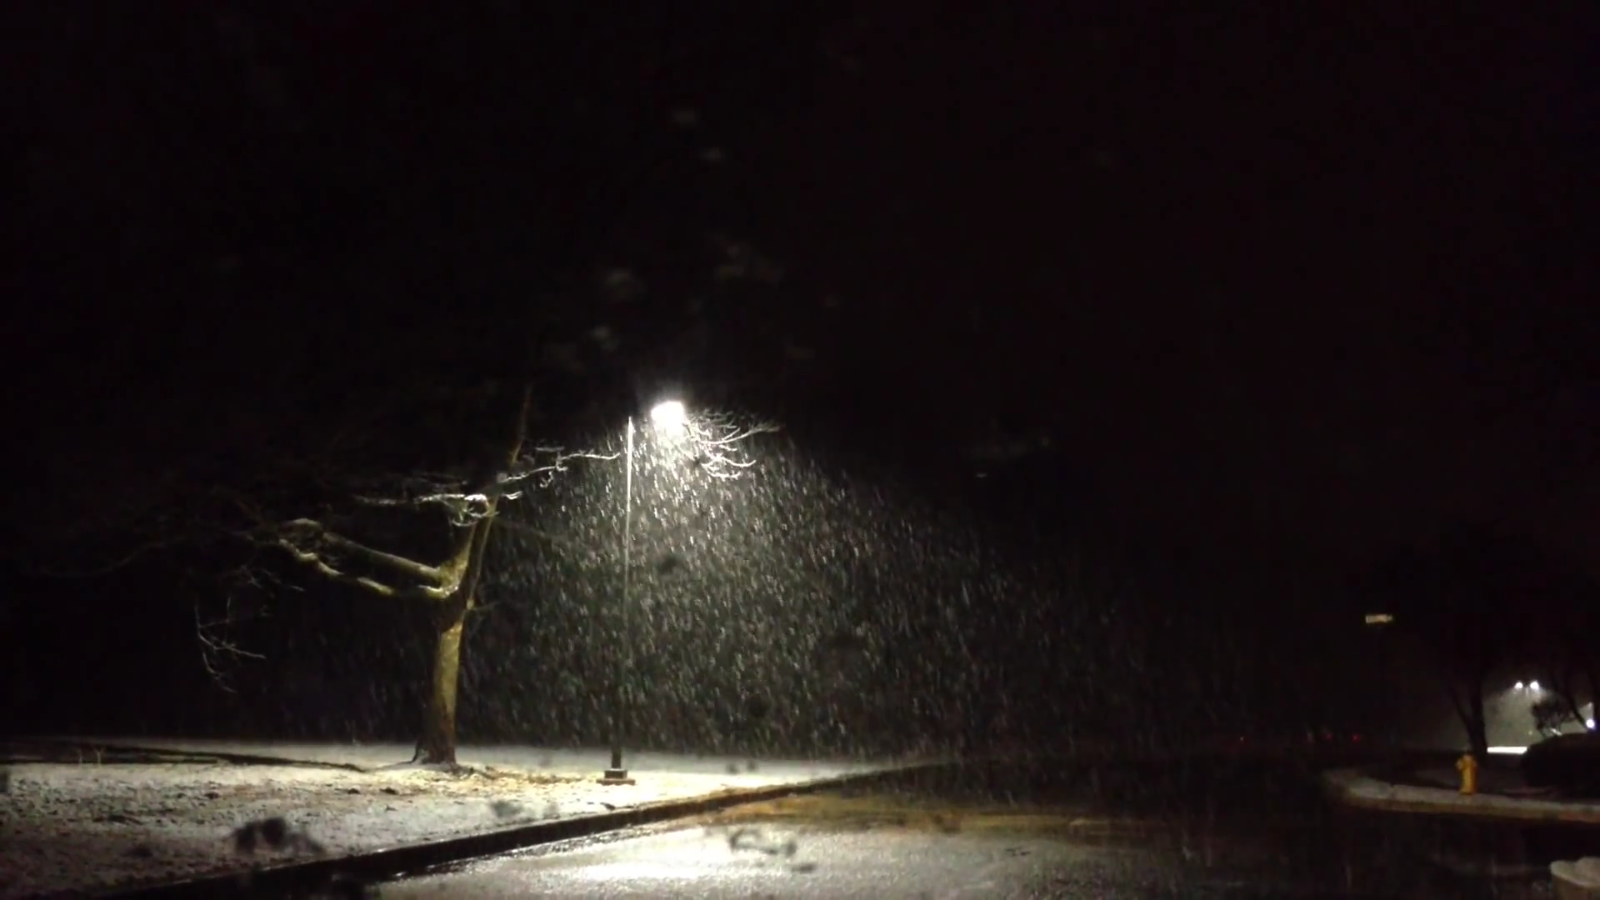
\includegraphics[width=0.9\textwidth]{youtube}
  \caption{\label{fig:youtube} Source: \href{https://www.youtube.com/watch?v=vHZb2xdVTCA}{https://www.youtube.com/watch?v=vHZb2xdVTCA}}
\end{figure}
\noindent
And off we went!



\section{Background}

In Figure~\ref{fig:youtube} and associated video we can identify a couple of elements being present:

\begin{enumerate}
  \item Models for trees and light posts.
  \item Multiple directed light cones.
  \item Snow on the ground.
  \item Snow tumbling through the air.
  \item Shadows cast on the ground.
  \item Snow stuck and falling on the camera lens.
  \item The camera shaking.
\end{enumerate}

All these has some crux, even the most simplest tasks like placing millions of little snow flakes on the screen. Lets look at them in order.


\subsection{Multiple directed light cones}

We looked into a couple of different techniques when it came to making the light:


\subsection{Snow on the ground}

There were some pretty sophisticated models used in the Disney film Frozen \href{https://disney-animation.s3.amazonaws.com/uploads/production/publication_asset/94/asset/SSCTS13_2.pdf}{[1]}, but we deemed them unfit for real time usage. Then again the reference image has no moving ground snow.


\subsection{Shadows}


\subsubsection{Shadow stensils}

\subsubsection{Shadow Maps}

Shadow maps are achieved by rendering a depth map from the viewport of the light source and then using it in the the shading of the real render from the camera viewport:

\begin{lstlisting}[label=lst:shadow-shaing,caption=How the shadow buffer is used to shade the real world.]
float getShadow() {
  vec4 shadowCoordinateWdivide = lightSourceCoord / lightSourceCoord.w;
  shadowCoordinateWdivide.z -= 0.002;
  float distanceFromLight = texture(shadowMap, shadowCoordinateWdivide.st).x;
    distanceFromLight = (distanceFromLight-0.5) * 2.0;
  float shadow = 1.0; // 1.0 = no shadow
  if (lightSourceCoord.w > 0.0)
    if (distanceFromLight < shadowCoordinateWdivide.z)
      shadow = 0.2;
  return shadow;
}
\end{lstlisting}



\subsection{Falling snow}

\subsubsection{Navier Stokes}

In order to simulate the effect of gusts of wind blowing on the snow navier stokes equations could be used \href{http://www.intpowertechcorp.com/GDC03.pdf}{[2]}. The linked paper is about fluid dynamics but since they're pretty much the same we're sure the methods described could still be applied.




\section{Implementation}

With 3200 fresh lines of code our solution is split up into 10 C files and 10 shader programs. We do geometry instancing for the particle systems, shadow maps for the projection of shadows and proximity based directed lighting.

Our code is organized so that each pair of shaders has a corresponding C-file which deals with all the specifics of that shader, each C-file exposes a single entry point for each shader with the complexities hidden away:

\begin{lstlisting}[label=lst:entry-points,caption= The entry points of each shader pair\, listed in decreasing complexity.]
void drawFull(Model *m, mat4 cameraTransform, mat4 modelTransform, mat4 shadowMapTransform, GLuint texture, GLuint shadowMap, struct Light* light, vec3 cameraPosition);
void drawModelInstanced(Model *m, mat4 camera, mat4 model, struct Light* light);
void drawSimple(Model *m, mat4 cameraTransform, mat4 modelTransform, GLuint texture);
void drawPlain(Model* m, mat4 modelViewProjectionTransform, mat4 modelTransform);
\end{lstlisting}

The most simple of our shaders called by \emph{drawPlain} takes only the pointer to a model, a transform from the model coordinate system to that of the camera, and finally a matrix for placing and morphing the model within the world.

If we take a walk into the function in Listing~\ref{lst:drawPlain} it does what you'd expect. The code for \emph{drawFull} and all the others are similarily dull.

\begin{lstlisting}[label=lst:drawPlain,caption= The contents of the drawPlain function.]
void drawPlain(Model *m, mat4 cameraTransform, mat4 modelTransform) {
  mat4 modelViewProjectionTransform = Mult(cameraTransform, modelTransform);

  glUseProgram(plainProgram);
  glUniformMatrix4fv(modelViewProjectionLocation, 1, GL_TRUE, modelViewProjectionTransform.m);

  // Vertex positions.
  glBindVertexArray(m->vao);
  glBindBuffer(GL_ARRAY_BUFFER, m->vb);
  glVertexAttribPointer(positionLocation, 3, GL_ GL_FALSE, 0, 0);
  glEnableVertexAttribArray(positionLocation);

  glDrawElements(GL_TRIANGLES, m->numIndices, GL_UNSIGNED_INT, 0L);
  printError("drawPlain()");
}
\end{lstlisting}

What might be of interest is the shader code itself, we'll get to that in the following chapters.


\subsection{Shadow maps}

Something which eased our work was the realization that a camera and a light source have a lot of commonalities:

\begin{lstlisting}[label=lst:lamp-struct,caption=Light source struct]
struct Camera {
  vec3 position;
  vec3 normal;
  vec3 target;
  mat4 projection;
};

struct Light {
  struct Camera camera;
  vec3 intensities;
  float ambientCoefficient;
  float coneAngle;
};
\end{lstlisting}

This made it possible for us to position and rotate the light sources using the normal FPS camera controls we had developed for the camera - merely storing the data kept in a camera and then using it for a light source.

Other than that there is nothing surprising in our implementation of shadow maps. We draw the the depth map with the simplest shader possible after which we use the resulting FBO.

Our implementation of shadow maps stems from (TODO: Matteus, minns du vad vi tog den ifrån?).

The vertex shaders does nothing interesting with the geometry, so we'll jump straight into the full fragment shader. In Listing~\ref{lst:shader-light-struct} we see the struct passed on to the shader.

\begin{lstlisting}[label=lst:shader-light-struct,caption= The light struct received in the shader.]
uniform struct Light {
  vec3 position;
  vec3 intensities;
  float ambientCoefficient;
  float coneAngle;
  vec3 coneDirection;
} light;
\end{lstlisting}

Using the data passed in as this structure we apply light if the texel is within the light cone.

\begin{lstlisting}[label=lst:applyLight,caption= Shader function for applying lighting]
vec3 applyLight(Light light, vec3 surfaceColor, vec3 normal,
    vec3 surfacePos, vec3 surfaceToCamera, float shadow) {
  float materialShininess = 1.0;
  vec3 materialSpecularColor = vec3(0.25);

  vec3 surfaceToLight = normalize(light.position - surfacePos);
  float distanceToLight = length(light.position - surfacePos);
  float attenuation = 1.0 / (0.1 + 0.0001 * pow(distanceToLight, 3));

  // Cone restrictions
  float lightToSurfaceAngle = degrees(acos(dot(-surfaceToLight,
    normalize(light.coneDirection))));
  if(lightToSurfaceAngle > light.coneAngle / 2) {
    attenuation = 0.0;
  }

  float diffuseCoefficient = max(0.0, dot(normal, surfaceToLight)
    * 0.5f + 0.5f);
  float specularCoefficient = diffuseCoefficient > 0 ?
    pow(max(0.0, dot(surfaceToCamera, reflect(-surfaceToLight,
      normal))), materialShininess) : 0;

  vec3 ambient = light.ambientCoefficient * surfaceColor.rgb
    * light.intensities;
  vec3 diffuse = diffuseCoefficient * surfaceColor.rgb
    * light.intensities;
  vec3 specular = specularCoefficient * materialSpecularColor
    * light.intensities;

  return ambient + shadow * attenuation * (diffuse + specular);
}
\end{lstlisting}

The last argument passed into the \emph{applyLight} function in Listing~\ref{lst:applyLight} is the output of the \emph{getShadow} function in Listing~\ref{lst:getShadow}.

\begin{lstlisting}[label=lst:getShadow,caption= The shader function figuring out whether the texel is in the shade.]
float getShadow() {
  vec4 shadowCoordinateWdivide = lightSourceCoord / lightSourceCoord.w;
  shadowCoordinateWdivide.z -= 0.002;
  float distanceFromLight = texture(shadowMap, shadowCoordinateWdivide.st).x;
  distanceFromLight = (distanceFromLight-0.5) * 2.0;
  float shadow = 1.0;
  if (lightSourceCoord.w > 0.0)
    if (distanceFromLight < shadowCoordinateWdivide.z) // shadow
      shadow = 0.2;
  return shadow;
}
\end{lstlisting}


\subsection{FBO debugging}

We implemented the display of FBO's so that we could see what was drawn into them. As we can see in Listing~\ref{lst:fbo-code} we're able to reuse our normal drawing code for the debugging.

\begin{lstlisting}[label=lst:fbo-code,caption= Switching between the FBO's]
int displayFBOKeyIsDown = keyIsDown('f');
if(displayFBOKeyWasDown && !displayFBOKeyIsDown)
  displayFBO = (displayFBO + 1) % (NR_STREET_LIGHTS + 1);
displayFBOKeyWasDown = displayFBOKeyIsDown;
if(displayFBO)
  drawSimple(modelPlane, Mult(S(.04, .04, .04), Rx(45)), IdentityMatrix(),
    fbos[displayFBO - 1]->depth);
\end{lstlisting}

This places a square in front of the camera displaying the depth buffer we want to inspect:

\begin{figure}[ht]
  \centering
  
\includegraphics[width=0.9\textwidth]{fbo}
  \caption{\label{fig:fbo-image} The depth buffer from a street light.}
\end{figure}




\section{Problems}

A lot, like you have no idea how many problems we had.

\subsection{Detangling global state}

We've probably refactored the codebase completelely somewhere around three times, trying to untangle it from iself. The code we started out with, mostly based on old lab and project code with

\subsection{Shadow buffer bugs}

We ended up wasting about a week trying to debug a fully working implementation of shadow maps, only that it didn't render correct on the specific hardware we were developing it on.


\section{Conclusions}

What we got was this:

\begin{figure}[ht]
  \centering
  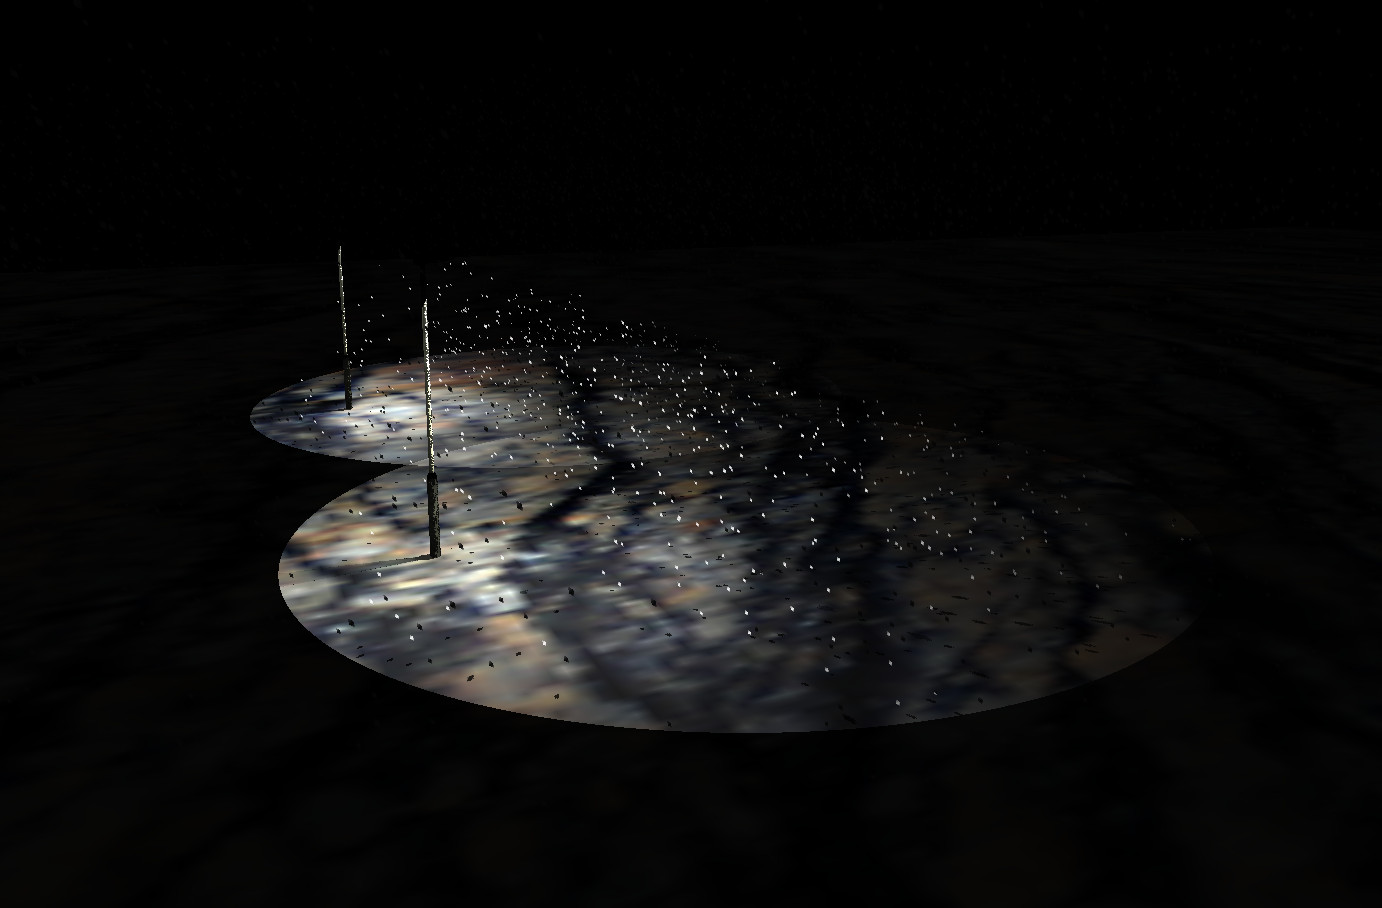
\includegraphics[width=0.9\textwidth]{result}
  \caption{\label{fig:label} Our OpenGL snow scene.}
\end{figure}

You can also see a short video on \href{YouTube}{TODO!}

\end{document}